Deux résistors, $R_1 = \qty{\v{R1}}{\ohm}$ et $R_2 = \qty{\v{R2}}{\ohm}$, sont branchés en parallèle sur une source de \qty{\v{U}}{V}.

\begin{center}
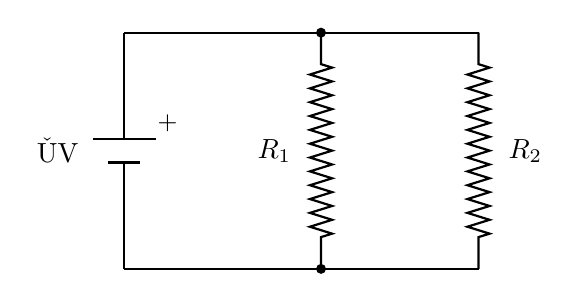
\begin{tikzpicture}[thick, res/.style={decorate,decoration={zigzag,segment length=5pt,amplitude=4pt,pre length=0.4cm,post length=0.4cm}}]
    \draw (0,0) -- (0,1.35);
    \draw (-0.2,1.35) -- (0.2,1.35);
    \draw (-0.4,1.65) -- (0.4,1.65);
    \draw (0,1.65) -- (0,3);
    \node[left] at (-0.45,1.5) {\qty{\v{U}}{V}};
    \node at (0.55,1.85) {\small$+$};
    \draw (0,3) -- (4.5,3);
    \draw (0,0) -- (4.5,0);
    \draw[res] (2.5,3) -- (2.5,0);
    \draw[res] (4.5,3) -- (4.5,0);
    \node[left] at (2.25,1.5) {$R_1$};
    \node[right] at (4.75,1.5) {$R_2$};
    \fill (2.5,3) circle (1.8pt); \fill (2.5,0) circle (1.8pt);
\end{tikzpicture}
\end{center}

\begin{enumerate}[label=\alph*)]
    \item Déterminez l'intensité du courant dans chaque résistor.
    \item Déterminez l'intensité du courant fourni par la source.
    \item Déterminez la résistance équivalente du circuit et vérifiez qu'elle est plus petite que la plus petite des deux résistances.
\end{enumerate}
